\title{On studying neural network expressiveness using topological data analysis and knot theory}

\author{Alexandre Louvet}

\documentclass[12pt]{article}
\usepackage[legalpaper, margin=2in]{geometry}

\usepackage{graphicx}
\usepackage{tikz}
\usetikzlibrary{decorations.markings}
\usepackage{amsmath}
\usepackage{tcolorbox}
\usepackage{enumitem}
\usepackage{multicol}
\usepackage{changepage}

\usepackage[utf8]{inputenc}
\usepackage{amsfonts}
\usepackage{stmaryrd}

\newfont{\titre}{cmr10 at 11pt}
\newfont{\soustitre}{cmbx10 at 11pt}
\newcommand{\N}{\mathbb{N}}
\newcommand{\Z}{\mathbb{Z}}
\newcommand{\Q}{\mathbb{Q}}
\newcommand{\R}{\mathbb{R}}
\newcommand{\C}{\mathbb{C}}
\newcommand{\U}{\mathbb{U}}
\newcommand{\F}{\mathcal{F}}
\renewcommand{\P}{\mathcal{P}}
\newcommand{\V}{\mathcal{V}}
\renewcommand{\d}{\, \mbox{d}}
\renewcommand{\H}{\mathcal{H}}
\newcommand{\B}{\mathcal{B}}
\renewcommand{\S}{\mathcal{S}}
\renewcommand{\L}{\mathcal{L}}
\newcommand{\M}{\mathcal{M}}
\newcommand{\GL}{\mbox{GL}}
\renewcommand{\O}{\mbox{O}}
\newcommand{\SO}{\mbox{SO}}
\renewcommand{\Im}{\mbox{Im} \,}
\newcommand{\Tr}{\mbox{Tr} \,}
\newcommand{\rg}{\mbox{rg} \,}
\newcommand{\Id}{\mbox{Id}}
\newcommand{\I}{\mbox{I}}
\newcommand{\sv}{\\[2pt]}
\newcommand{\Sv}{\\[6pt]}
\newcommand{\SV}{\\[9pt]}
\newcommand{\rv}{\\[-6pt]}
\newcommand{\chapitre}{\section*}
\newcommand{\paragraphe}{\subsection*}
\newcommand{\partie}{\subsubsection*}
\newcommand{\debut}{\\[-14pt] \begin{itemize} \parskip -3pt}
\newcommand{\fin}{\end{itemize}}
\let \[ = \llbracket
\let \] = \rrbracket
\def\overcirc #1 {\buildrel \circ \over #1 \ }
\def\bar #1{\hskip1pt\overline{\hskip-1pt#1}\hskip1pt}
\def\interieur #1{{\mathop{#1}\limits^{\circ}}}   % interieur
\def\adherence #1{\hskip1pt\overline{\hskip-1pt#1\hskip1pt}\hskip-1pt} % adherence
\def\modulo #1{\ \left[ #1 \right]}               % modulo
\def\eqv{\mathop{\sim}\limits}                    % equivalence
\def\vct#1{\hskip1pt\overrightarrow{\hskip-1pt#1\hskip1pt}\hskip-1pt} % vecteur
\def\rac#1#2{\root {\scriptstyle #1} \of {#2}}    % racine
\def\dcap {\bigcap\limits}            % intersection
\def\dcup {\bigcup\limits}            % union
\def\dlim  {\lim\limits}              % limite (lim)
\def\dprod {\prod\limits}             % produit
\def\dsum  {\sum\limits}              % somme
\def\dint  {\displaystyle\int}        % integrale

\parindent = 0mm


\newtheorem{theorem}{Theorem}
\newtheorem{lemma}{Lemma}
\newtheorem{proposition}{Proposition}
\newtheorem{scolium}{Scolium} 
\newtheorem{definition}{Definition}
\newenvironment{proof}{{\sc Proof:}}{\hfill $\square$}
\newenvironment{AMS}{}{}
\newenvironment{keywords}{}{}

\def\layersep{2.5cm}

\begin{document}
\newpage
\maketitle
\begin{abstract}
  In this paper we summarize the state of the art on the question of neural network expressiveness both on the theoretical approach to the problem with the study of universal approximators and some practical approaches using topological data analysis and trajectories. We then propose an analysis of the question from a knot theory perspective and share results using studied methods for datasets in dimension 3 and 4.
\end{abstract}

\newpage

\tableofcontents

\newpage

\section{Neural network expressiveness}

\subsection{Definition}

Let $I_n$ denote the $n$-dimensional unit cube $[0,1]^n$ and $\F(I_n,\R)$ be the space of functions from $I_n$ to $\R$. We want to study the density of the subsets $S_f$ of $\F(I_n,\R)$ that can be written as follows:\\

\begin{center}
  $S_f = \{G_N(x) \in \F(I_n,\R) \mid G(x) = \sum\limits_{i=1}^{N} \alpha_i f(y_j^T x + \theta_j )\}$, $N \in \N $
\end{center}

depending on the choice of $f \in \F(\R,\R)$. In the previous equation $y_j \in \R^n$ and $\alpha_j, \theta \in \R$, $y^T$ is the transpose of y and $y^Tx$ is the inner product of $y$ and $x$.\\

The study of neural network expressiveness consists of the problem described above when $f$ is a function used as an activation function for neural network. The study of density can be on the whole set $\F(I_n,\R)$ or on subsets of it such as $\C(I_n,\R)$ the set of continuous functions from $I_n$ to $\R$.\\

In particular if $S_f$ is dense in a subset $A \subseteq \F(I_n, \R)$ we will say that a single-layer feed-forward neural network (Fig. 1) with $f$ as its activation function is a \textit{universal approximator} of $A$. Considering a neural network has a finite number of nodes neural network expressiveness also consists of the study of the rate of approach of the approximation, i.e. the sudy of \\

\begin{center}
  $\lim\limits_{N \to \infty} H(N) = \max\limits_{h\in A} (\min\limits_{G_n \in S_f} (\parallel G_n - h \parallel))$ with $\parallel . \parallel$ the canonical norm on $\F(I_n, \R)$
\end{center}

The study of that limit and especially of its asympatotic approximation gives an idea of the efficiency of the approximator, i.e. the amount of node to add to the network to improve the approximation.\\

\begin{center}
  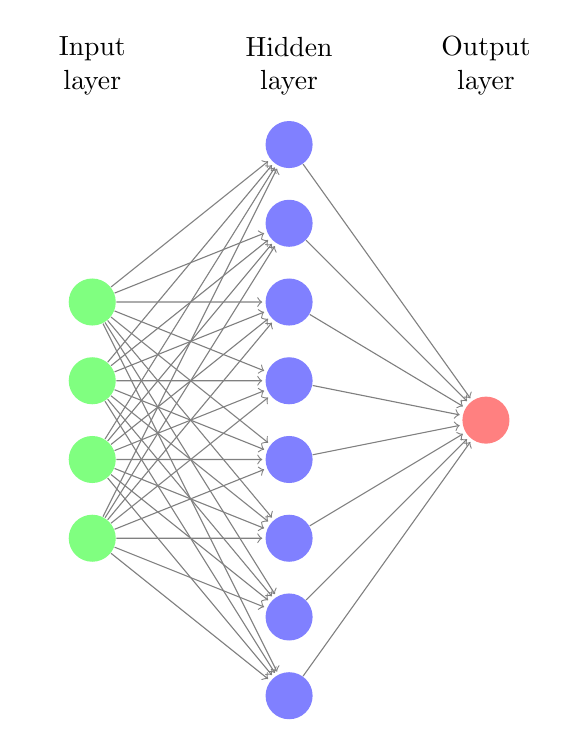
\begin{tikzpicture}[shorten >=1pt,->,draw=black!50, node distance=\layersep]
      \tikzstyle{every pin edge}=[<-,shorten <=1pt]
      \tikzstyle{neuron}=[circle,fill=black!25,minimum size=17pt,inner sep=0pt]
      \tikzstyle{input neuron}=[neuron, fill=green!50];
      \tikzstyle{output neuron}=[neuron, fill=red!50];
      \tikzstyle{hidden neuron}=[neuron, fill=blue!50];
      \tikzstyle{annot} = [text width=4em, text centered]

      % Draw the input layer nodes
      \foreach \name / \y in {1,...,4}
      % This is the same as writing \foreach \name / \y in {1/1,2/2,3/3,4/4}
      \node[input neuron] (I-\name) at (0,-\y) {};

      % Draw the hidden layer nodes
      \foreach \name / \y in {1,...,8}
          \path[yshift=2.0cm]
              node[hidden neuron] (H-\name) at (\layersep,-\y cm) {};

      % Draw the output layer node
      \node[output neuron, right of=H-5,yshift=0.5cm] (O) {};

      % Connect every node in the input layer with every node in the
      % hidden layer.
      \foreach \source in {1,...,4}
          \foreach \dest in {1,...,8}
              \path (I-\source) edge (H-\dest);

      % Connect every node in the hidden layer with the output layer
      \foreach \source in {1,...,8}
          \path (H-\source) edge (O);

      % Annotate the layers
      \node[annot,above of=H-1, node distance=1cm] (hl) {Hidden layer};
      \node[annot,left of=hl] {Input layer};
      \node[annot,right of=hl] {Output layer};
  \end{tikzpicture}\\
Fig 1: A single-layer feed-forward neural network with $n=4$ and $N=8$
\end{center}

\subsection{Universal Approximator}

In this section we will study the different subsets on which the logistic and ReLU functions acts as universal approximators.\\ 

\subsubsection{Sigmoidal functions}

We say that a function $\sigma \in \F(I_n, \R)$ is a sigmoidal function if:\\

\begin{center}
  $\sigma(x) \to
  \begin{cases}
    0 &\text{as $t \to +\infty$}\\
    1 &\text{as $t \to -\infty$}
  \end{cases}$
\end{center}

The sigmoidal functions include the logistic function defined as:\\

\begin{center}
  $f(x) = \frac{1}{1+e^{-x}}$
\end{center}

widely used as an activation function for neural networks.\\

The first study of neural network expressiveness with sigmoidal functions date back to by G.Cybenko in 1989 \cite{cybenko_approximation_1989}. He proves that $S_\sigma$ for $\sigma$ a sigmoidal function is dense in regards of the supremum norm in $C(I_n, \R)$. The demonstration goes as follows.\\

We denote $M(I_n)$ the space of signed regular Borel measures on $I_n$\\

\begin{definition}
  $\sigma$ \text{is discriminatory if} $\mu \in M(I_n)$ \text{and}\\ 
  \begin{center}
  $\forall y \in \R^n,$ $\theta \in \R \int\limits_{I_n} \sigma(y^Tx + \theta) d\mu(x) = 0 \implies \mu = 0$
\end{center}
\end{definition}

\begin{theorem}
  Let $\sigma$ be a contininuous discriminatory function. Then finite sums of the form\\\begin{center}
    $G(x) = \sum\limits_{i=1}^N \alpha_i \sigma(y^Tx + \theta_i)$
  \end{center}
  are dense in $C(I_n, \R)$
\end{theorem}

\begin{proof}
  Let $S \subset C(I_n)$ be the set of the function of the form $G(x)$. S in a linear subset of $C(I_n)$. Let us show that the closure of $S$ is $C(I_n)$.\\
  Assume it is not the case. Then the closure of $S$, denoted $R$, is a proper subspace of $C(I_n)$. Using the Hahn-Banach theorem, there esists $L$ a bounded linear functional on $C(I_n)$ with $L \ne 0$ and  $L(R) = L(S) = 0$\\
  Using the Riesz Representation Theorem, we obtain:\\
  \begin{center}
    $L(h) = \int\limits_{I_n} h(x)d\mu(x)$
  \end{center}
  for some $\mu \in M(I_n)$, for all $h\in C(I_n)$. Since $\sigma(y^Tx + \theta_i)  \in R$, we have\\
  \begin{center}
    $\forall y, \theta \int\limits_{I_n} \sigma(y^Tx + \theta) d\mu(x) = 0$
  \end{center}
  Since $\sigma$ is discriminatory, we have $\mu = 0$ and $L = 0$ follows!
  Hence the closure of $S$ is $C(I_n)$ and by definition $S$ is dense in $C(I_n)$
\end{proof}\\
\Sv
  Now let us show that sigmoidal functions are discriminatory.
  \begin{lemma}
    Any bounded, measurable sigmoidal function, a, is discriminatory. In particular, any continuous sigmoidal function is discriminatory.
  \end{lemma}

  \begin{proof}
    First note $\forall x,y,\theta, \phi$ 
\begin{center}
  $\sigma_\lambda(x) = \sigma(\lambda (y^Tx + \theta) + \phi)
  \begin{cases}
    \to 1 &\text{for $y^Tx+\theta > 0$ as $\lambda \to +\infty$}\\
    \to 0 &\text{for $y^Tx+\theta < 0$ as $\lambda \to +\infty$}\\
    =\sigma(\phi) & \text{for $y^Tx+\theta = 0$}
  \end{cases}$
\end{center}
Thus $\sigma_\lambda(x)$ converges pointwise and boundedly to:

\begin{center}
  $\gamma(x)
  \begin{cases}
    =1 &\text{for $y^Tx+\theta > 0$}\\
    =0 &\text{for $y^Tx+\theta < 0$}\\
    =\sigma(\phi) & \text{for $y^Tx+\theta = 0$}
  \end{cases}$
\end{center}
as $\lambda \to +\infty$\\
\sv
Let $\Pi_{y,\theta} = \{x \mid y^Tx+\theta = 0\}$ and let $H_{y,\theta} = \{x \mid y^Tx + \theta > 0\}$. Lesbegue bounded convergence theorem gives us:\\
\begin{center}
  $0 = \int\limits_{I_n}\sigma_\lambda(x)d\mu(x)$\\
  $ = \int\limits_{I_n} \gamma(x)d\mu(x)$\\
  $\sigma(\phi)\mu(\Pi_{y,\theta}) + \mu(H_{y,\theta})$
\end{center}
for all $\phi, \theta, y$\\
\sv
Fix $y$, we write \\
\begin{center}
  $F(h) = \int_{I_n}h(y^Tx)d\mu(x)$
\end{center}
Note that $F$ is a bounded function on $L^\infty(\R)$ since $\mu$ is a signed mesure. By chosing  $h$ as the indicator function on $[\theta, \infty[$, we have:
\begin{center}
  $F(h) = \int_{I_n} h(y^Tx) d\mu(x) = \mu(\Pi_{y,-\theta}) + \mu(H_{y,-\theta}) = 0$
\end{center}
By linearity $F(h) = 0$ for indicator function on any interval and hence for any simple function (sum of indicator functions) and since simple functions are dense in $L^{\infty}(\R), F = 0$.
In particular it is true for the bounded function $s(u) = sin(m.u)$ and $c(u) = cos(m.u)$. It gives:
\begin{center}
  $F(s+ic) = \int_{I_n} cos(m^Tx) + i sin(m^Tx) d\mu(x) = \int_{I_n} exp(im^Tx)d\mu(x) = 0$
\end{center}
for all $m$. Therefore the fourier transform of $\mu$ is 0 and $\mu$ must be 0. Hence $\sigma$ is discriminatory.
  \end{proof}\\

  This proves that any function of $C(I_n, \R)$ can be approximated by a single-layer network with sigmoidal functions as activation function.\\

  In 1991, Hornik extended in \cite{hornik_approximation_1991} gave the proof for bounded non-constant functions of $F(I_n,\R)$. The proof is very similar to the original one.\\

\subsubsection{ReLU functions}

ReLU functions stands for Rectified Linear Units, there are formed of two pieces of linear functions. They gained interest recently by showing convincing results in a lot of different applications.\\ 

In 2016 Arora et al. \cite{arora_understanding_2018} showed a version of the universal approximation theorem for piecewise linear function that includes ReLU functions.\\

\begin{definition}
  We say a function $f: \R^n \to \R$ is continuous piecewise linear (PWL) if there exists a finite set of polyhedra whose union is $\R^n$, and $f$ is affine linear over each polyhedron (implies continuity because affine regions are closed and cover $\R^n$)
\end{definition}

\begin{proposition}
  Every function in $L^q(\R^n), (1 \le q \le \infty)$ can be arbitrarily approximated in the $L^q$ norm (which for a function $f$ is given by $||f||_q = (\int |f|^q)^{1/q}$) by a ReLU Deep Neural Network.
\end{proposition}

\begin{proof}

  We know that any ReLU DNN represents a PWL function, let's prove the converse.\\
  \sv
  By theorem 1 in \cite{wang_generalization_2005} any piecewise linear function $f: \R^n \to \R$, can be written:\\
  \begin{center}
    $f = \sum\limits_{j=1}^{p}s_j(\max\limits_{i\in S_j} l_i)$
  \end{center}
  with $l_i$ $(i\le i \le k)$ linear functions, $S_i$ $(1 \le i \le p) \subseteq \{1, ..., k\}$ with $\forall i, |S_i| \le n + 1$ and $\forall j \in \{1,...,p\},  s_j \in \{-1, +1\}$ \\
  \sv
  It means that any PWL convex function can be represented as a linear combination of at most $n+1$ affine pieces. That's to say a ReLU DNN with size $n+1$.\\
  \SV
  Let $p \in \N^*$, let $f \in L^p(\R^n)$, consider the function sequence:\\
  \begin{center}
    $f_n(x) = (x - \frac{k}{n})f(\frac{k}{n}) + (1 - x + \frac{k}{n})f(\frac{k+1}{n})$ with $\frac{k}{n} \le x < \frac{k+1}{n}, n \ge 1$ 
  \end{center}

  $f_n \xrightarrow[n \to \infty]{} f$, and $\forall n, f_n$ is a PWL continous function. Therefore the continuous PWL functions are dense in $L^p(\R^n)$.
  \SV
  Since any PWL function $\R^n \to \R$ is representable by a ReLU DNN, unniversal approximation theorem follows from the fact that the family of continuous PWL functions is dense in any $L^p(\R^n)$ space for $1 \le p \le \infty$. 
  
\end{proof}\\
\SV
In this article, Arora et al. also give a higher bound for the depth of the network. they show that the network required for any function $f \in L^q(\R^n)$ is at most $\lceil log_2(n+1) \rceil$.\\

In 2018, Hannin \& Selke \cite{hanin_approximating_2018} showed that the minimal width a ReLUneural network must have in order to approximate any function $f: \R^n \to \R^m$ is $n + m$. Giving a lower bound to the width of the ReLU network.

\newpage
\thispagestyle{empty}
\mbox{}
\newpage

\section{Homology}

The study of homology is part of the field of algebraic topology. We will first introduce the concept of homology, then take a look at the theoretical concept behind it by introducing $\Delta$-complex: a primitive topolgical structure that allow the study of homology. Then with the introduction of simplicial homology and finally singular homology we will complete the presentation of the fundamental objects used in the study of homolgy. We will then reconsider these tools in the context of our research. This part heavily relies on the book \textit{Algebraic Topolgy} by A. Hatcher \cite{hatcher_algebraic_2002} and the class given by P. Albin at University of Illinois \cite{albin_1_2018} with the same book as class material. 

\subsection{The idea of homology}

\begin{center}
  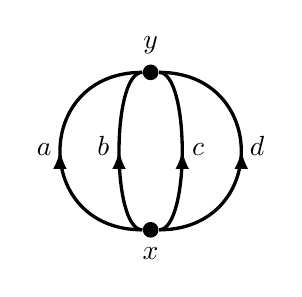
\begin{tikzpicture}[node distance={20mm}] 
    \node[circle,fill,inner sep=2pt, label=below:{$x$}] (1) {}; 
    \node[circle,fill,inner sep=2pt, label=above:{$y$}] (2) [above of=1] {}; 
\begin{scope}[very thick,decoration={
    markings,
    mark=at position 0.5 with {\arrow{latex}}}
    ] 
    \draw[postaction={decorate}] (1) .. controls +(left:1.5cm) and +(left:1.5cm) .. (2)
\foreach \p in {$a$} {node[sloped,above,pos=0.5,rotate=-90, xshift=-0.2cm, yshift=-0.2cm]{\p}};
 \draw[postaction={decorate}, fill=white] (1) .. controls +(left:0.5cm) and +(left:0.5cm) .. (2)
\foreach \p in {$b$} {node[sloped,above,pos=0.5,rotate=-90, xshift=-0.2cm, yshift=-0.2cm]{\p}};
 \draw[postaction={decorate}] (1) .. controls +(right:0.5cm) and +(right:0.5cm) .. (2)
\foreach \p in {$c$} {node[sloped,above,pos=0.5,rotate=-90, xshift=0.2cm, yshift=-0.2cm]{\p}};
 \draw[postaction={decorate}] (1) .. controls +(right:1.5cm) and +(right:1.5cm) .. (2)
\foreach \p in {$d$} {node[sloped,above,pos=0.5,rotate=-90, xshift=0.2cm, yshift=-0.2cm]{\p}};
\end{scope}
\end{tikzpicture} 
\end{center}

Consider the space $X_1$ in the figure drawn above. We can see two points $x$ and $y$ as well as four edges $a$, $b$, $c$ and $d$. Consider the loops formed by travelling along the edges, for instance the path $ab^{-1}$ is a loop with $x$ as the basepoint. Something to consider is that the loop $b^{-1}a$ is basically the same loop but starting from a different basepoint, $y$ in that case. By abelianizing, we can consider cycles instead of loops without any basepoint.\\

The abelian groups having only one operation, we will then switch to additive notations to remain in accordance with Hatcher's notations. With that new notation we can write equalities such as $(a-c) + (b-d) = (a-d) + (b-c)$. This is justified by the fact that from an algebraic point of view, there is no difference between these two cycles.\\

Let us call any linear combination of edges, chains. Then the condition for a chain $ka + lb + mc + nd$ with $k,l,m,n \in \N$ to be a cycle is $k + l + m + n = 0$.\\

Now let us start to formalize these concepts. Consider $C_0$ the free abelian group spanned by the vertices $x,y$ and let $C_1$ be the free abelian group spanned by the edges $a,b,c,d$. One can define an homomorphism $\delta: C_1 \to C_0$ that sends any basis element of $C_1$ to $x-y$. Thus we have $\delta(ka+lb+mc+nd) = (k+l+m+n)a - (k+l+m+n)y$ and $ker(\delta) = \{$ cycles of $X_1$ $\}$. $\{ a-b, b-c, c-d \}$ forms a basis for this kernel, i.e. any cycle is a linear combination of the most obvious cycles of $X_1$, that conveys the information that $X_1$ has three visibles "holes" formed by the space between its four edges.\\

\begin{center}
  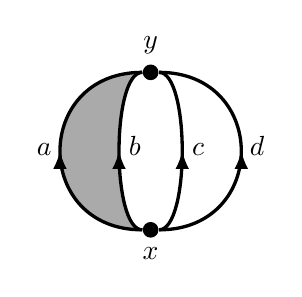
\begin{tikzpicture}[node distance={20mm}] 
    \node[circle,fill,inner sep=2pt, label=below:{$x$}] (1) {}; 
    \node[circle,fill,inner sep=2pt, label=above:{$y$}] (2) [above of=1] {}; 
\begin{scope}[very thick,decoration={
    markings,
    mark=at position 0.5 with {\arrow{latex}}}
    ] 
    \draw[postaction={decorate}, fill={rgb:black,1;white,2}] (1) .. controls +(left:1.5cm) and +(left:1.5cm) .. (2)
      \foreach \p in {$a$} {node[sloped,above,pos=0.5,rotate=-90, xshift=-0.2cm, yshift=-0.2cm] (3) {\p}};
 \draw[postaction={decorate}, fill=white] (1) .. controls +(left:0.5cm) and +(left:0.5cm) .. (2)
   \foreach \p in {$b$} {node[sloped,above,pos=0.5,rotate=-90, xshift=0.2cm, yshift=-0.2cm] (4) {\p}};
 \draw[postaction={decorate}] (1) .. controls +(right:0.5cm) and +(right:0.5cm) .. (2)
\foreach \p in {$c$} {node[sloped,above,pos=0.5,rotate=-90, xshift=0.2cm, yshift=-0.2cm]{\p}};
 \draw[postaction={decorate}] (1) .. controls +(right:1.5cm) and +(right:1.5cm) .. (2)
\foreach \p in {$d$} {node[sloped,above,pos=0.5,rotate=-90, xshift=0.2cm, yshift=-0.2cm]{\p}};
\end{scope}
\end{tikzpicture} 
\end{center}

Now fill the hole between edges $a$ and $b$ with a 2-cell, namely $A$ to create a new space $X_2$. Considering it as being oriented clockwise, its boundary is $a-b$. The cycle $a-b$ is homotopic to a point since it can now be contracted by sliding over $A$, it no longer encloses a hole in G. That suggests that homology should consider only the quotient group of what we found previously by $a-b$. In this quotient group the cycles $a-c$ and $b-c$ are equivalent. Which is consistent with the fact that they are homotopic in $X_2$.\\

Algebraically we can now consider a pair of homomorphism $\delta_1, \delta_2$ such that $C_2 \xrightarrow{\delta_2} C_1 \xrightarrow{\delta_1} C_0$ where $C_2$ is the cyclic group spanned by $A$ and $\delta_2(A) = a-b$. The quotient group we are interrested in is $ker(\delta_1)/Im(\delta_2)$, i.e. the 1-dimensional cycles modulo those that are boundaries. We will call it the homology group $H_1(X_2)$. I can also be computed in $X_1$ by considering $C_2$ to be zero since there are no two cells in $X_2$. $H_1(X_2)$ now only admits two generators $b-c$ and $cd$ expressing the geometric fact that the number of holes reduced from 3 to 2.\\


\begin{center}
  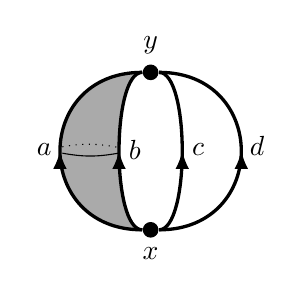
\begin{tikzpicture}[node distance={20mm}] 
    \node[circle,fill,inner sep=2pt, label=below:{$x$}] (1) {}; 
    \node[circle,fill,inner sep=2pt, label=above:{$y$}] (2) [above of=1] {}; 
\begin{scope}[very thick,decoration={
    markings,
    mark=at position 0.5 with {\arrow{latex}}}
    ] 
    \draw[postaction={decorate}, fill={rgb:black,1;white,2}] (1) .. controls +(left:1.5cm) and +(left:1.5cm) .. (2)
      \foreach \p in {$a$} {node[sloped,above,pos=0.5,rotate=-90, xshift=-0.2cm, yshift=-0.2cm] (3) {\p}};
 \draw[postaction={decorate}, fill=white] (1) .. controls +(left:0.5cm) and +(left:0.5cm) .. (2)
   \foreach \p in {$b$} {node[sloped,above,pos=0.5,rotate=-90, xshift=0.2cm, yshift=-0.25cm] (4) {\p}};
 \draw[postaction={decorate}] (1) .. controls +(right:0.5cm) and +(right:0.5cm) .. (2)
\foreach \p in {$c$} {node[sloped,above,pos=0.5,rotate=-90, xshift=0.2cm, yshift=-0.2cm]{\p}};
 \draw[postaction={decorate}] (1) .. controls +(right:1.5cm) and +(right:1.5cm) .. (2)
\foreach \p in {$d$} {node[sloped,above,pos=0.5,rotate=-90, xshift=0.2cm, yshift=-0.2cm]{\p}};
\end{scope}
\draw[dotted] (3) to [out=10, in=170] (4);
\draw (3) to [out=350, in=190] (4);
\end{tikzpicture} 
\end{center}

Suppose we attach another 2-cell between $a$ and $b$ to create $X_3$, namely $B$. $C_2$ now consists of linear combinations of $A$ and $B$ and $\delta_2(A) = \delta_2(B) = a-b$. In the one hand, $H_1(X_3) = H_1(X_2) \approx \Z \times \Z$, but this time $ker(\delta_2) \neq 0$ and $A-B$ is its generator, hence we have $H_2(X_3) = ker(\delta_2) \approx \Z$. Topologically the cycle $A-B$ is equivalent to a sphere and it detects the presence of a "hole" enclosed by this sphere rather than a circle.\\

The pattern we can see appear with these examples is rather clear. The n-cell complexes of $X$ forms free abelian groups $C_n(X)$ and one can define homomorphisms $\delta_n: C_n \to C_{n-1}$ to define homology groups $H_n(X) = ker(\delta_n)/Im(\delta_{n+1})$. The only problem now is to define $\delta_n$ for any $n$. If it is simple for small $n$ (head minus tail for a vertex), it becomes rather complicated when $n$ grows and more complex polyhedral cells appear in $X$. The most efficient approach is to decompose polyhedra into simplices which allows simple orientation and boundary computation. For that purpose we will define nice cellular complexes that will be the fundamental element for homology computation in the homology theories presented after. 

\subsection{$\Delta$-complexes}

The most important theory of algebraic topology is called simplicial homology, since it is technically complicated we will first introduce a simpler version of it called simplicial homology. The natural definition spaces of simplicial homology is called $\Delta$-complexes that we will introduce in this part.\\

The projective plane, the klein bottle and the torus can be obtained from squares by identifying edges and giving them orientation as draw below.

\tcbset{top=0pt,right=10pt,left=10pt,bottom=0pt,nobeforeafter, colframe=blue!75!black,colback=white,fonttitle=\bfseries,center title}
\begin{center}
  \tcbox[title=$T$]{
  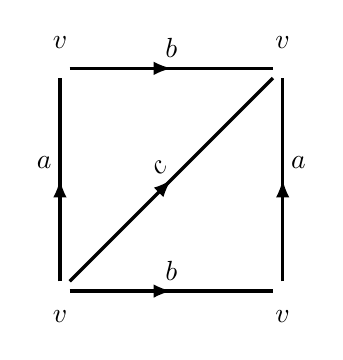
\begin{tikzpicture}[node distance={20mm}] 
    \node[draw=none, label={}] (1) {}; 
    \node[draw=none, label={$v$}] (2) [above right of=1] {}; 
    \node[draw=none, label={$v$}] (3) [above left of=1] {}; 
    \node[draw=none, label=below:{$v$}] (4) [below right of=1] {}; 
    \node[draw=none, label=below:{$v$}] (5) [below left of=1] {}; 
\begin{scope}[very thick,decoration={
    markings,
    mark=at position 0.5 with {\arrow{latex}}}
    ] 
    \draw[postaction={decorate}] (3) -- (2)
      \foreach \p in {$b$} {node[sloped,above,pos=0.5,rotate=0] (6) {\p}};
    \draw[postaction={decorate}] (4) -- (2)
      \foreach \p in {$a$} {node[sloped,above,pos=0.5,rotate=-90, xshift=0.2cm] (7) {\p}};
    \draw[postaction={decorate}] (5) -- (4)
      \foreach \p in {$b$} {node[sloped,above,pos=0.5,rotate=0] (8) {\p}};
    \draw[postaction={decorate}] (5) -- (3)
      \foreach \p in {$a$} {node[sloped,above,pos=0.5,rotate=-90, xshift=-0.2cm] (9) {\p}};
    \draw[postaction={decorate}] (5) -- (2)
      \foreach \p in {$c$} {node[sloped,above,pos=0.5,rotate=0] (10) {\p}};
\end{scope}
      
\end{tikzpicture} 
}
\hspace{0.5cm}
\tcbox[title=$\R P^2$]{
  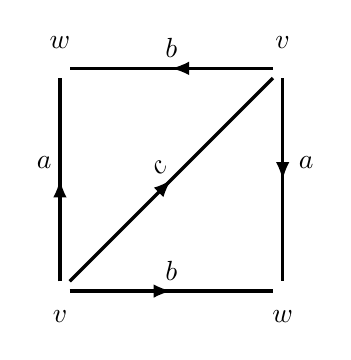
\begin{tikzpicture}[node distance={20mm}] 
    \node[draw=none, label={}] (1) {}; 
    \node[draw=none, label={$v$}] (2) [above right of=1] {}; 
    \node[draw=none, label={$w$}] (3) [above left of=1] {}; 
    \node[draw=none, label=below:{$w$}] (4) [below right of=1] {}; 
    \node[draw=none, label=below:{$v$}] (5) [below left of=1] {}; 
\begin{scope}[very thick,decoration={
    markings,
    mark=at position 0.5 with {\arrow{latex}}}
    ] 
    \draw[postaction={decorate}] (2) -- (3)
      \foreach \p in {$b$} {node[sloped,above,pos=0.5,rotate=0] (6) {\p}};
    \draw[postaction={decorate}] (2) -- (4)
      \foreach \p in {$a$} {node[sloped,above,pos=0.5,rotate=90, xshift=0.3cm] (7) {\p}};
    \draw[postaction={decorate}] (5) -- (4)
      \foreach \p in {$b$} {node[sloped,above,pos=0.5,rotate=0] (8) {\p}};
    \draw[postaction={decorate}] (5) -- (3)
      \foreach \p in {$a$} {node[sloped,above,pos=0.5,rotate=-90, xshift=-0.2cm] (9) {\p}};
    \draw[postaction={decorate}] (5) -- (2)
      \foreach \p in {$c$} {node[sloped,above,pos=0.5,rotate=0] (10) {\p}};
\end{scope}
\end{tikzpicture}
}
\hspace{0.5cm}
\tcbox[title=$K$]{
  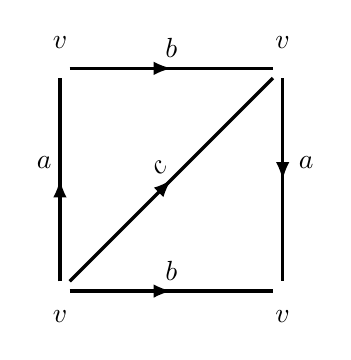
\begin{tikzpicture}[node distance={20mm}] 
    \node[draw=none, label={}] (1) {}; 
    \node[draw=none, label={$v$}] (2) [above right of=1] {}; 
    \node[draw=none, label={$v$}] (3) [above left of=1] {}; 
    \node[draw=none, label=below:{$v$}] (4) [below right of=1] {}; 
    \node[draw=none, label=below:{$v$}] (5) [below left of=1] {}; 
\begin{scope}[very thick,decoration={
    markings,
    mark=at position 0.5 with {\arrow{latex}}}
    ] 
    \draw[postaction={decorate}] (3) -- (2)
      \foreach \p in {$b$} {node[sloped,above,pos=0.5,rotate=0] (6) {\p}};
    \draw[postaction={decorate}] (2) -- (4)
      \foreach \p in {$a$} {node[sloped,above,pos=0.5,rotate=90, xshift=0.3cm] (7) {\p}};
    \draw[postaction={decorate}] (5) -- (4)
      \foreach \p in {$b$} {node[sloped,above,pos=0.5,rotate=0] (8) {\p}};
    \draw[postaction={decorate}] (5) -- (3)
      \foreach \p in {$a$} {node[sloped,above,pos=0.5,rotate=-90, xshift=-0.2cm] (9) {\p}};
    \draw[postaction={decorate}] (5) -- (2)
      \foreach \p in {$c$} {node[sloped,above,pos=0.5,rotate=0] (10) {\p}};
\end{scope}
\end{tikzpicture}
}
\end{center}

In fact any closed surface can be constructed this way, i.e. by cutting a polygon along its diagonals and identifying pairs of edges. The idea between $\Delta$-complexes is to generalize this idea to any dimension. The n-dimensional analog of the triangle is called the n-simplex.This is the smallest convex set in a Euclidean space $\R^m$ containing $n + 1$ points $v_0 , ... , v_n$ that do not lie in a hyperplane of dimension less than $n$. The points $v_i$ are the vertices of the simplex and the simplex is denoted $[v_0, ..., v_n]$. The standard n-simplex is:\\

\begin{center}
  $\Delta^n = \{ (t_0,...t_n) \in \R^{n+1} \mid \sum_i t_i  = 1$ and $t_i \ge 0$ for all $i \}$
\end{center}

Its vertices are the unit vectors along the coordinate axes.\\

It is important to keep track of an ordering for the vertices and an n-simplex will always be considered with an ordering for its vertices. This will allow us to give an orientation for its edges $[v_iv_j]$ with respect to the ordering of the indices. It also determines a canonical linear homeomorphism from the standart n-simplex $\Delta^n$ into any other n-simplex preserving the order of the vertices: $(t_0, ..., t_n) \mapsto \sum_i t_i v_i$. The corfficients are the barycentric coordinates of the points $sum_i t_i v_i$ in $[v_0, ..., v_n]$.\\

If we delete one of the vertices of an n-simplex $[v_0, ..., v_n]$, the remaining n vertices span an (n-1)-simplex, called face of $[v_0, ..., v_n]$ that will conventionnaly keep the same orientation as in $[v_0, ..., v_n]$. The union of all the face of $\Delta^n$ is the boundary of $\Delta^n$, noted $\delta \Delta^n$. The open simplex $\mathring{\Delta}^n$ is $\Delta^n - \delta \Delta^n$, is the interior of $\Delta^n$.\\

A $\Delta$-complex on a topological space $X$ is a collection of maps $\sigma_\alpha : \Delta^n \to X$  with the following properties:\\

\begin{enumerate}[label=(\roman*)]
  \item The restriction $\sigma_\alpha \mid \mathring{\Delta}^n$ is injective, and each point of $X$ is in the image of exactly one such restriction $\sigma_\alpha \mid \mathring{\Delta}^n$.
  \item Each restriction if $\sigma_\alpha$ to a face of $\Delta^n$ is one if the maps $\sigma_\beta : \Delta^{n-1} \to X$ (identifying the face of $\Delta^n$ with the face of $\Delta^{n-1}$ using the canonical linear homeomorphism between them and preserving the vertices ordering).
  \item A set $A \subset X$ is open if and only if $\sigma_\alpha^{-1}(A)$ is open in $\Delta^n$ for each $\sigma_\alpha$.
\end{enumerate}

The earlier decompositions of the torus, projective plane, and Klein bottle into two triangles, three edges, and one or two vertices allow well-definess of associated $\Delta$-complex structures with a total of six $\sigma_\alpha$'s for the torus and Klein bottle and seven for the projective plane. The orientation of edges are compatible with an ordering of the vertices (example below). This ordering determines the maps $\sigma_\alpha$.

\begin{center}
\tcbox[title=$\R P^2$]{
  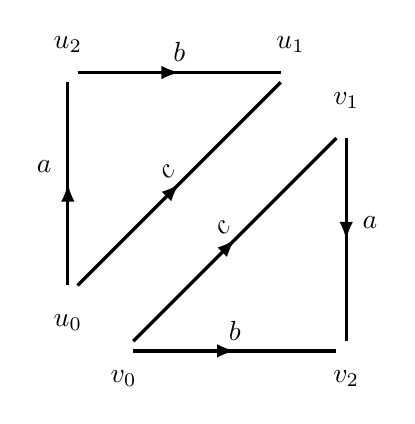
\begin{tikzpicture}[node distance={10mm}] 
    \node[draw=none, label={}] (1) {}; 
    \node[draw=none, label={}] (2) [below left of=1] {}; 
    \node[draw=none, label={}] (3) [below right of=1] {}; 
    \node[draw=none, label={}] (4) [above right of=1] {}; 
    \node[draw=none, label=below:{$v_0$}] (5) [below left of=2] {}; 
    \node[draw=none, label=below:{$v_2$}] (6) [below right of=3] {}; 
    \node[draw=none, label={$v_1$}] (7) [above right of=4] {}; 
    \node[draw=none, label={}] (8) [above left of=1] {}; 
    \node[draw=none, label={}] (9) [below left of=8] {}; 
    \node[draw=none, label={}] (10) [above left of=8] {}; 
    \node[draw=none, label={}] (11) [above right of=8] {}; 
    \node[draw=none, label={$u_1$}] (12) [above right of=11] {}; 
    \node[draw=none, label={$u_2$}] (13) [above left of=10] {}; 
    \node[draw=none, label=below:{$u_0$}] (14) [below left of=9] {}; 
\begin{scope}[very thick,decoration={
    markings,
    mark=at position 0.5 with {\arrow{latex}}}
    ] 
    \draw[postaction={decorate}] (5) -- (6)
      \foreach \p in {$b$} {node[sloped,above,pos=0.5,rotate=0] (17) {\p}};
    \draw[postaction={decorate}] (7) -- (6)
      \foreach \p in {$a$} {node[sloped,above,pos=0.5,rotate=90, xshift=0.3cm] (15) {\p}};
    \draw[postaction={decorate}] (5) -- (7)
      \foreach \p in {$c$} {node[sloped,above,pos=0.5,rotate=0] (16) {\p}};
    \draw[postaction={decorate}] (14) -- (13)
      \foreach \p in {$a$} {node[sloped,above,pos=0.5,rotate=-90, xshift=-0.3cm] (18) {\p}};
    \draw[postaction={decorate}] (13) -- (12)
      \foreach \p in {$b$} {node[sloped,above,pos=0.5,rotate=0] (19) {\p}};
    \draw[postaction={decorate}] (14) -- (12)
      \foreach \p in {$c$} {node[sloped,above,pos=0.5,rotate=0] (20) {\p}};
\end{scope}
\end{tikzpicture}
}
\end{center}

\subsection{Simplicial homology}

Let us now define the simplicial homology groups of a $\Delta$-complex $X$. Let $\Delta_n(X)$ be the free abelian group with basis the open $n$-simplices $e^n_\alpha$ of $X$. The elements of $\Delta_n(X)$ are called n-chains and are of the form $\sum_\alpha n_\alpha e^n_\alpha$ with $n_\alpha \in \Z$. Equivalently, this could be written as $\sum_\alpha n_\alpha \sigma_\alpha$ where $\sigma_\alpha : \Delta^n \to X$ is the characteristic map of $e^n_\alpha$ with image the closure of $e^n_\alpha$. Such a sum can be considered as a finite collection, or "chain", of $n$-simplices in $X$.\\

The boundary of the $n$-simplex $[v_0, ..., v_n]$ consists of the various $(n-1)$-dimensional simplices $[v_0, ... , \hat{v_i} , ... , v_n]$ (indicates all $v_{k}, 1 \le k \le n$ but $i$). We might wish that the boundary of  $[v_0, ..., v_n]$ be the $(n-1)$-chain formed by the sum of the faces $[v_0, ... ,\hat{v_i} , ... , v_n]$. It turns out to be betters to insert sign to take into account orientations. It allow to coherently orient all the faces of the simplex. That is why we let the boundary be $\sum_i (-1)^i [v_0, ... , \hat{v_i} , ... , v_n]$.\\


\tcbset{colback=white,colframe=black,top=10mm,bottom=10mm}
\begin{tcolorbox}
\begin{multicols}{2}
  \begin{center}
  \begin{tikzpicture}[node distance={20mm}] 
    \node[draw=none, label={}] (1) {}; 
    \node[draw=none, label=right:{$v_1$}] (2) [above right of=1] {}; 
    \node[draw=none, label=left:{$v_0$}] (3) [above left of=1] {}; 
\begin{scope}[very thick,decoration={
    markings,
    mark=at position 0.5 with {\arrow{latex}}}
    ] 
    \draw[postaction={decorate}] (3) -- (2)
      \foreach \p in {} {node[sloped,above,pos=0.5,rotate=90, xshift=0.3cm] (5) {\p}};
\end{scope}
\end{tikzpicture}
\\
  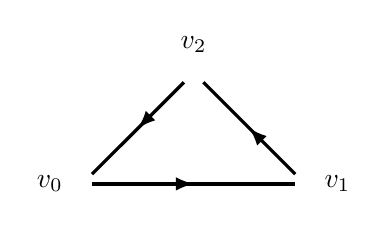
\begin{tikzpicture}[node distance={20mm}] 
    \node[draw=none, label={$v_2$}] (1) {}; 
    \node[draw=none, label=right:{$v_1$}] (2) [below right of=1] {}; 
    \node[draw=none, label=left:{$v_0$}] (3) [below left of=1] {}; 
\begin{scope}[very thick,decoration={
    markings,
    mark=at position 0.5 with {\arrow{latex}}}
    ] 
    \draw[postaction={decorate}] (1) -- (3)
      \foreach \p in {} {node[sloped,above,pos=0.5,rotate=0] (4) {\p}};
    \draw[postaction={decorate}] (3) -- (2)
      \foreach \p in {} {node[sloped,above,pos=0.5,rotate=90, xshift=0.3cm] (5) {\p}};
    \draw[postaction={decorate}] (2) -- (1)
      \foreach \p in {} {node[sloped,above,pos=0.5,rotate=0] (5) {\p}};
\end{scope}
\end{tikzpicture}
\end{center}
\begin{center}


\columnbreak

$\delta [v_0,v_1] = [v_1] - [v_0]$\\
\vspace{2.3cm}

$\delta [v_0, v_1, v_2] = [v_1, v_2] - [v_0, v_2] + [v_0, v_1]$

\end{center}
\end{multicols}
\end{tcolorbox}
\\

We define a boundary homomorphism for a general $\Delta$-complex $X$, $\delta_n : \Delta_n (X) \to \Delta_{n-1} (X)$ by specifying its values on the absis elements:\\

\begin{center}

  $\delta_n(\sigma_\alpha) = \sum_i (-1)^i \sigma_\alpha \mid [v_0 , ... , \hat{v_i} , ... , v_n]$

\end{center}

The image set of $\delta_n$ is $\Delta_{n-1} (X)$ since each restriction $\sigma_\alpha \mid [v_0 , ... , \hat{v_i} , ... , v_n]$ is the caracteristic map of an $(n-1)$-simplex of $X$.\\

\begin{lemma}

  The composition $\Delta_n (X) \xrightarrow{\delta_n} \Delta_{n-1} (X) \xrightarrow{\delta_{n-1}} \Delta_{n-2} (X)$ is zero.

\end{lemma}

\begin{proof}

  We have $\delta_n(\sigma) = \sum_i (-1)^i \sigma \mid [v_0, ... , \hat{v_i} , ... , v_n] $, hence \\
  \vspace{-10pt}
  \begin{center}
  $\delta_{n-1}\delta_n (\sigma) = \sum\limits_{j < i} (-1)^i (-1)^j \sigma \mid [v_0, ... , \hat{v_j} , ... , \hat{v_j} , ... , v_n]$
  \sv
$+ \sum\limits_{j > i} (-1)^i (-1)^{j-1} \sigma \mid [v_0, ... , \hat{v_i}, ... , \hat{v_j} , ... , v_n] = 0$.
\end{center}

  The last equality comes from the switch of $i$ and $j$ in the second sum.

\end{proof}
\\

We end up with a sequence of homomorphisms of abelian groups:\\

\begin{center}
  $... \to C_{n+1} \xrightarrow{\delta_{n+1}} C_n \xrightarrow{\delta_n} C_{n-1} \to ... \to C_1 \xrightarrow{\delta_1} C_0 \xrightarrow{\delta_0} 0$
\end{center}

with $\delta_n\delta_{n+1} = 0$ for each $n$ (cf Lemma 2).We call such a sequence a chain complex. The equation $\delta_n \delta_{n+1} = 0$ is equivalent to the inclusion Im $\delta_{n+1} \subset$ Ker $\delta_n$. We can define the $n^{th}$ homology group of the chain complex to be the quotient group $H_n =$ Ker $\delta_n$/Im $\delta_{n+1}$. The elements of Ker $\delta_n$ are called cycle and elements of Im $\delta_{n+1}$ are called boundaries.Elements of $H_n$ are cosets of Im $\delta_{n+1}$ called homology classes. Two cycles representing the same homology class are said to be homologous, it means their difference is a boundary.\\

In the case of $C_n = \Delta_n(X)$, the homology group Ker $\delta_n$/Im$\delta_{n+1}$ will be denoted $H^\Delta_n(X)$ and called the $n^{th}$ simplicial homology group of $X$. \\

Example: Let us take $X = T$, the torus with the $\Delta$-complex structure pictured in section \textbf{2.2}. For recall, the structure has one vertex $v$, three edges $a, b, c$ and two 2-simplices $U$ and $V$. $\delta_1 = v - v = 0$ so $H_0^\Delta(X) \approx \Z$. Since $\delta_2 U = a + b - c = \delta_2 L$ and $\{a, b, a+ b - c\}$ is a basis for $\Delta_1(T)$, $H_1^\Delta(X) = \frac{\Delta_1(X)}{\delta_2(U)}$, it follows that $H_1^\Delta(X) \approx \Z \oplus \Z$ with basis the homology classes $[a]$ and $[b]$. Since there are no 3-simplices, $H_2^\Delta(T)$ is equal to Ker$\delta_2$, which is infinite cyclic generated by $U-L$ since $\delta(pU+qL) = (p+q)(a+b-c) = 0$ iff $p = -q$.\\
Therefore:\\
\begin{center}
  $H_n^\Delta(X) \approx
  \begin{cases}
    \Z \oplus \Z &\text{for $n=1$}\\
    \Z &\text{for $n=0,2$}\\
    0 &\text{for $n\ge3$}
  \end{cases}$
\end{center}

A $\Delta$-complex structure can be otained on $S^n$ by taking two copies of $\Delta^n$ and identifying boundaries using the identity map. Using previous notations, we have Ker$\delta_n$ an infinite cycle generated by $U-L$. Therefore $H_n^\Delta(S^n) \approx \Z$.\\

The simplicial homology is defined for simplical complexes. These are the $\Delta$-complexed whose simplices are uniquely determined by their vertices. Each $n$-simplex has $n+1$ distinct vertices and no other $n$-simplex has the same set of vertices. A simplicial complex can be described as a set $X_0$ of vertices and sets $X_n$ of $n$-simplices which are $(n+1)$-elements subsets of $X_0$. It is required that each $(k+1)$-element subset of the vertices of an $n$-simplex in $X_n$ is a $k$-simplix in $X_k$.\\

Compared with $\Delta$-complexes, simplicial complexes require more computation. For example a simplicial complex structure for the torus would require 14 triangles, 21 edges and 7 vertices. It can be shown that any $\Delta$-complex can be subdivided in a simplical complex.\\

\subsection{Singular homology}

\subsection{Homology in our research}

Homology exists as a computable alternative homotopy.

\newpage
\thispagestyle{empty}
\mbox{}
\newpage

\section{Topological data Analysis}

\subsection{Fundamental concepts}

\subsection{Persistent homology}

\newpage
\thispagestyle{empty}
\mbox{}
\newpage

\section{Knot theory}

\subsection{Definition}

\subsection{Knot determinant}

\subsubsection{Definition}

\subsubsection{Algorithms}

\newpage
\thispagestyle{empty}
\mbox{}
\newpage

\section{Measuring neural network expressiveness}

\subsection{Using topological data analysis}

\subsection{Using trajectories}

\newpage
\thispagestyle{empty}
\mbox{}
\newpage

\section{The study of trajectories from a knot theory perspective}

\subsection{Methodology}

\subsection{Algorithms}

\subsection{Results}

\newpage
\thispagestyle{empty}
\mbox{}
\newpage

\section{Extending the study of expressiveness with topological data analysis} 
\subsection{Methodology}

\subsection{Algorithms}

\subsection{Results}

\newpage
\thispagestyle{empty}
\mbox{}
\newpage

\bibliography{bibliography}

\bibliographystyle{ieeetr}

\end{document}

